\newpage
\section{Environment Considerations}
\label{app:envs}
In this work, we consider environments where zero-shot generalization is difficult, so the agent must learn through trial and error. We also want environments where overfitting to any particular task is difficult to ensure our method is general. A final practical consideration is that we consider environments wher across-episodic histories can be feasibly modeled with a causal transformer. Given these considerations, our evaluation environments need to satisfy three criteria:

\begin{enumerate}
\item {\it Supports many tasks:} The environments must be multi-task to ensure that our agent and the baselines do not overfit to any single task and instead is able to in-context reinforcement learn across many tasks within a given domain.

\item {\it Task must be hard to infer:} To ensure that the downstream tasks are hard to generalize to in zero-shot, we use environments that require exploration. Namely, we require environments where either the task can only be inferred from the reward and not the observation, or tasks that are partially observable.

\item {\it Supports multi-episodic contexts:} Lastly, we impose a practical constraint - the environment episodes must be short enough such that a normal GPT-like transformer can fit multiple episodes in its context. Since this work introduces \name as a method, we wish to investigate it in the cleanest possible setting using a canonical architecture. We leave investigating \name with more complex architectures that scale to longer sequences for future work.
\end{enumerate}

Prior related works~\citep{chen2021dt, lee2022mgdt, janner2021tto, reed2022gato} evaluated on Atari, OpenAI gym, and as well as other environments. However, Atari and OpenAI gym don't satisfy at least one of the above criteria. Atari and OpenAI gym episodes are often long and can contain thousands or more transitions per episode, so it's technically challenging to populate a causal transformer's context with across-episode histories. Indeed, the prior related works only considered within-episode context lengths. Additionally, it is often easy to infer the task from either the observation or the dense reward alone in both Atari and OpenAI gym, which reduces the need for exploration. For these reasons, we evaluate in environments that satisfy all three criteria instead.

\section{Closely Related Prior Methods}
\label{app:baselines}

In our main results we use Expert Distillation (ED) as a baseline. Here, we discuss how the most closely related methods differ from \name and why ED is sufficient to support the paper's claims. 

\noindent{\it Expert Distillation (ED):} ED is most similar to Gato~\citep{reed2022gato}, which models expert sequences from a converged RL policy using a causal transformer. ED also trains a causal transformer to predict actions using expert policy data. There are two key differences between ED and Gato. First, unlike Gato which utilizes small (relative to an episode length) within-episode contexts, ED is trained on the same across-episode contexts as \namenospace, so the architectures used by ED and \name are the same. The benefits of \name cannot therefore be attributed to across-episode contexts alone but also learning progress in the offline data used to train \namenospace. Second, ED models state-action-reward sequences while Gato models only state-action sequences. The main difference between ED and \name is that \name is trained on full multi-task learning histories rather than expert policy data.

\noindent {\it Decision Transformer (DT)~\citep{chen2021dt} and Multi-Game Decision Transformer~\citep{lee2022mgdt}:} DTs learn return-conditioned policies from single-task offline data collected by an RL agent. While the training data itself (an RL agent's replay buffer) contains learning, the context sizes used in DT are too small to capture any learning progress or identify the task using across-episode information. For instance, the Atari experiments use a context of length $30-50$ tokens, or $10-17$ transitions. Atari games can have hundreds or thousands of transitions in a single episode, which means these contexts capture mostly within-episode information. Additionally, very little learning progress happens in the underlying replay buffer data within that many transitions. 

Another difference between DT and \name / ED is that DT learns a return-conditioned model whereas \name / ED are both reward-conditioned. In our setting return-conditioning alone cannot yield an optimal policy since the agent does not know the task until after it explores the environment and can identify it using across-episode contexts. Since (i) DT uses small within-episodic contexts and (ii) return-conditioning would not help in the environments considered, this baseline is similar to ED with a small within-episode context which is strictly weaker than the long across-episode context variant of ED we consider.

\noindent {\it Trajectory Transformer (TTO)~\citep{janner2021tto}:} Like \namenospace, TTO also models state-action-reward tokens but in addition to predicting actions it also learns a world model by predicting states and rewards. To maximize return, TTO then uses beam search to select high-reward actions. However, in our setting, TTO will run into the same problem as DT. To model rewards accurately it will need longer across-episodic contexts since one environment supports many tasks. Similar to DT, MGDT, and Gato, TTO uses smaller within-episode contexts. For this reason, TTO will fare no better than DT, MGDT, or ED in the settings we consider. We also note that in contrast to TTO, \name is model-free. In \namenospace, actions are sampled from the transformer history-conditioned predictions and return maximization emerges from modeling the learning histories of an RL algorithm.

To summarize, \name differs from prior methods mainly because its context is across-episodic and hence large enough to capture learning progress and task information. \name could further be augmented by learning world models like TTO or conditioning on returns like DT, but these investigations would be well suited for future work since they are tangential to the main research question addressed in this work -- whether in-context RL can emerge by imitating the learning histories of an RL algorithm with long across-episodic contexts. %Augmenting \name with world models and return-conditioning would be interesting for future work but is tangential to the claims made in this work.

\name is also closely related to prior work in in-context meta-RL. While both \name and in-context meta-RL model across-episodic histories with memory-based architectures, prior in-context meta-RL algorithms, such as RL2~\citep{duan2016rl2} are trained online and rely on learning multi-episodic value functions with TD learning while \name is trained offline and uses a supervised imitation learning objective. 

\section{Expert Distillation Main Results}

We elaborate further on the main results in Fig.~\ref{fig:main_exps} and provide intuition regarding the behaviors of the ED baseline.  In Dark Room, Dark Room (Hard), and Watermaze, ED performance is either flat or it degrades. The reason for this is that ED only saw expert trajectories during training, but during evaluation it needs to first explore (\ie \, perform non-expert behavior) to identify the task. This required behavior is out-of-distribution for ED and for this reason it does not reinforcement learning in-context. In Dark Key-to-Door the agent is reset randomly at the beginning of each episode, whereas in all of the environments the agent's starting position is fixed. Due to random resets, the ED agent is sometimes reset by the first goal in Dark Key-to-Door which allows it to occasionally identify the first goal of the task, which is why it shows slight improvement.


\section{Model Size}
 We investigate how transformer capacity affects performance in Fig.~\ref{fig:analysis}. While in-context RL emerges across all model sizes investigated, we find that increasing the model depth, the model width in terms of embedding dimension, and (to a lesser extent) the number of attention heads improves performance on Dark Key-to-Door.


\begin{figure}[h]
  \begin{center}
    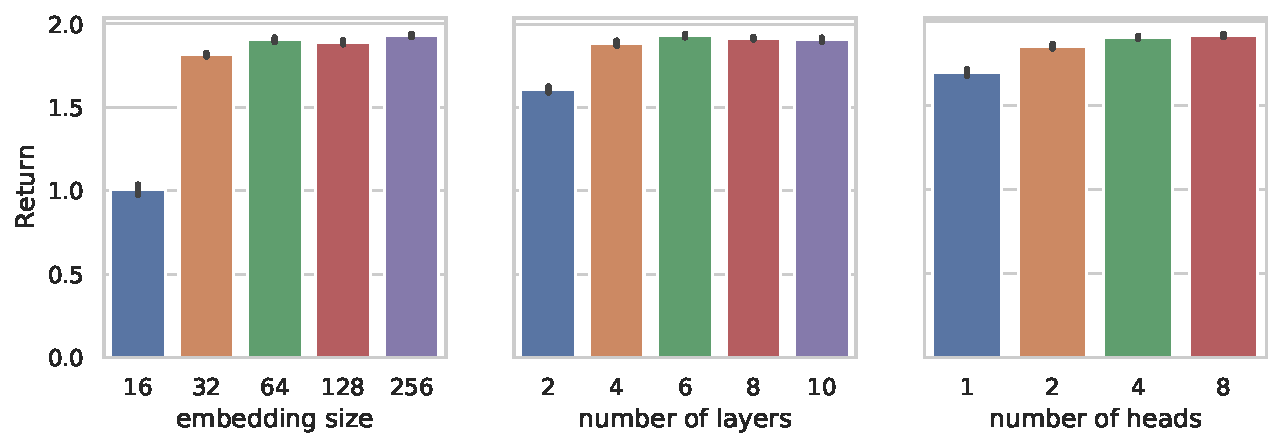
\includegraphics[width=0.6\textwidth]{assets/images/model_size_ablation.pdf}
  \end{center}
  \caption{\small {\it Model size investigations:} We investigate how increasing model capacity affects \namenospace. While in-context RL with \name emerges regardless of the model capacity, increasing the model depth and width helps improve \name until it achieves near-optimal performance. \looseness=-1}
\label{fig:analysis}
  %\vspace{-5mm}

\end{figure}

\newpage 

\section{Source Algorithm Training Runs}
\label{app:source}


\begin{figure}[h]

\centering
\begin{subfigure}{0.23\textwidth}
    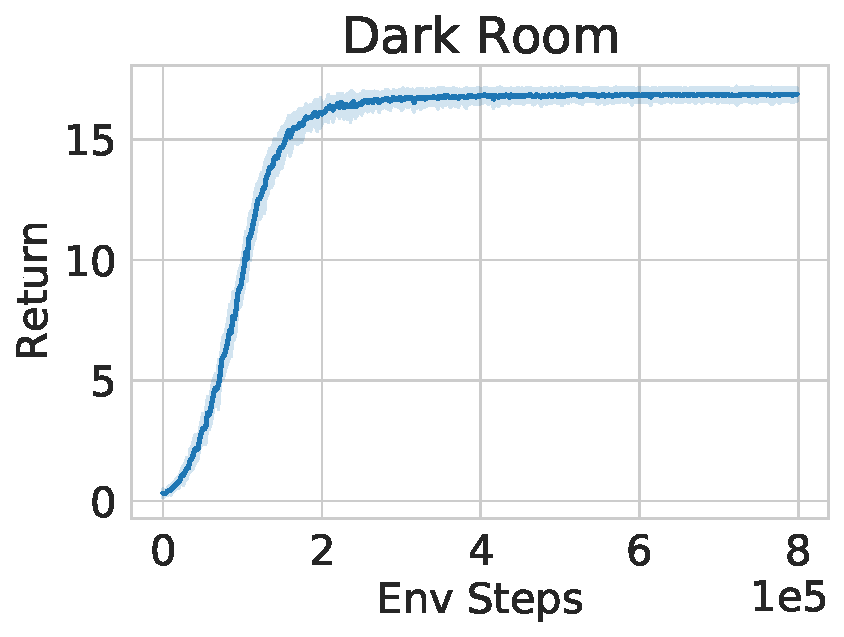
\includegraphics[width=\textwidth]{assets/images/9x9_1g_dense_source.pdf}
 
\end{subfigure}
\hfill
\begin{subfigure}{0.23\textwidth}
    %%EP.9.21: there's a purple curve not in the legend
    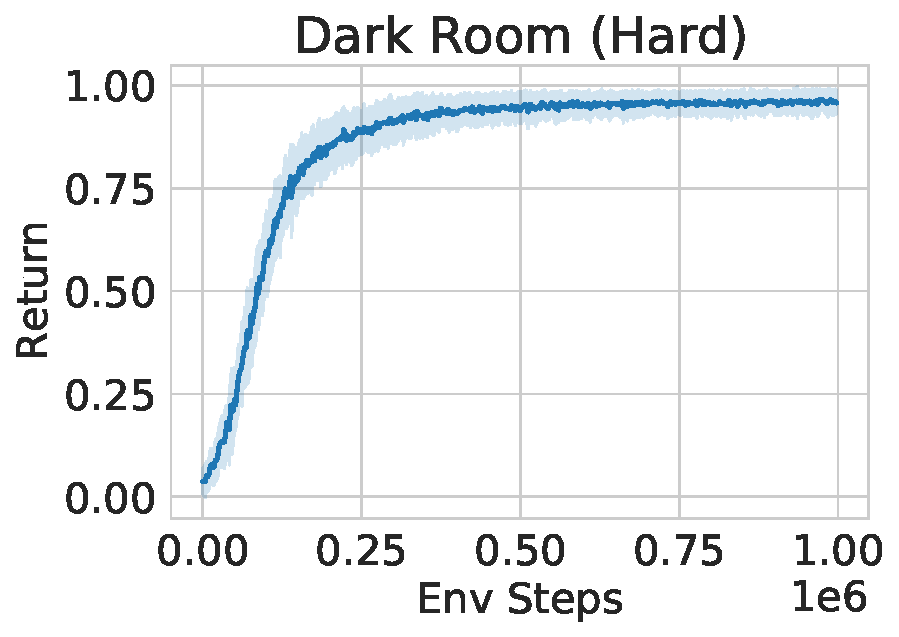
\includegraphics[width=\textwidth]{assets/images/17x17_1g_sparse_source.pdf}
 
\end{subfigure}
\hfill
\begin{subfigure}{0.23\textwidth}
    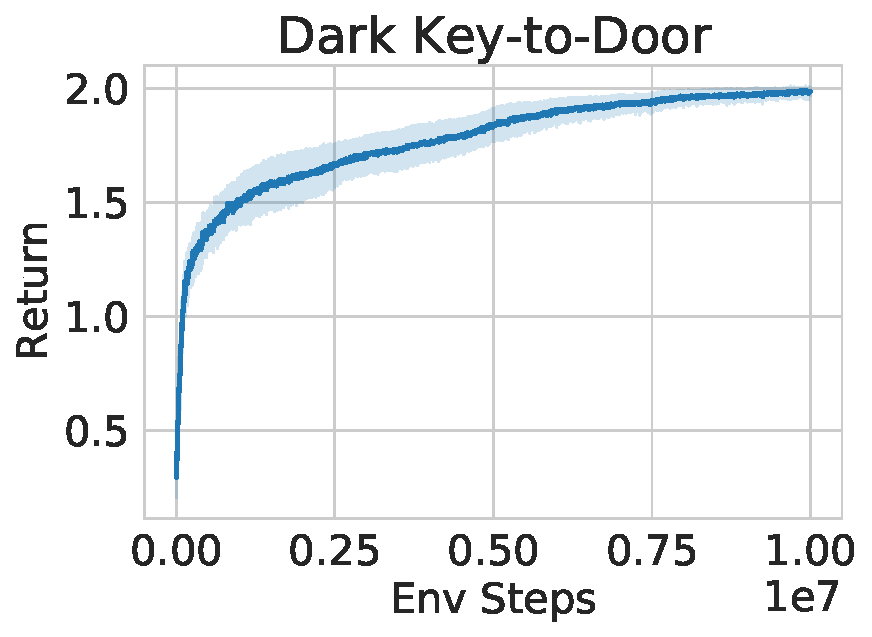
\includegraphics[width=\textwidth]{assets/images/9x9_2g_sparse_source.pdf}

\end{subfigure}
\hfill 
\begin{subfigure}{0.24\textwidth}
    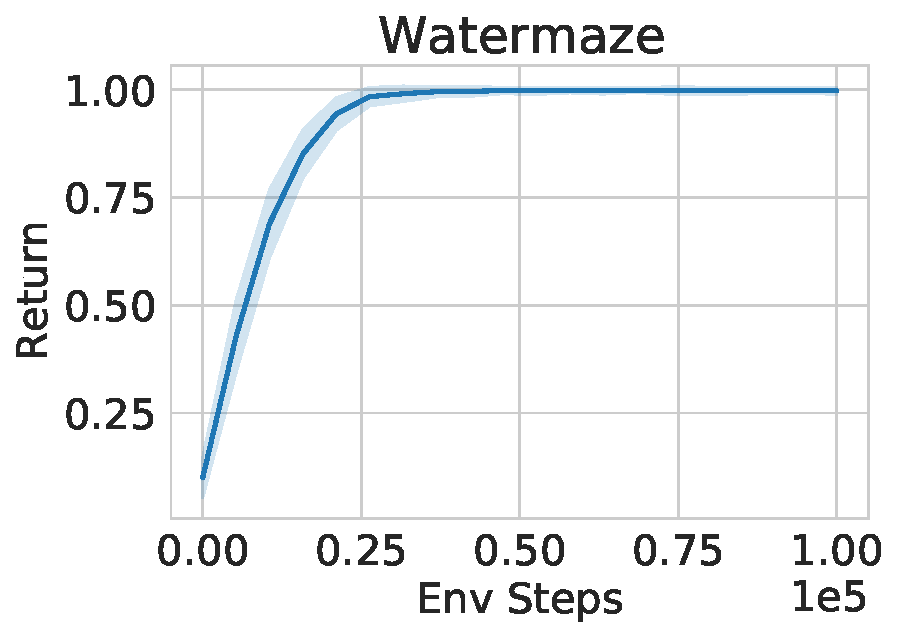
\includegraphics[width=\textwidth]{assets/images/watermaze_source.pdf}
 
\end{subfigure}
\caption{\small Asymptotic performance of the A3C~\citep{mnih16a3c} and a Q-$\lambda$ variant of the DQN~\citep{mnih2013dqn} RL algorithms used to produce learning histories for the Dark and Watermaze environments. These curves show the learning histories \name is trained on. The source algorithms plotted in Fig.~\ref{fig:main_exps} are the same as in these plots. \looseness=-1}
\label{fig:source}
\end{figure}




%\newpage


\section{Label Smoothing Ablation}
For the harder exploration task of Dark Room (Hard), we found that adding label smoothing regularization~\citep{szegedy2016inception,muller19labelsmoothing} improved the in-context learning ability of \name. In Figure~\ref{fig:label_smoothing_ablation} we ablate the benefit of using label smoothing for 3 different $\alpha$ values as well as with it turned off. Each curve in the figure denotes average performance over 5 training seeds. We can see that adding label smoothing up to a point improves the in-context learning ability of~\fullnamenospace, with performance continually increasing with the number of evaluation episodes. 

\begin{figure}[h!]
\centering
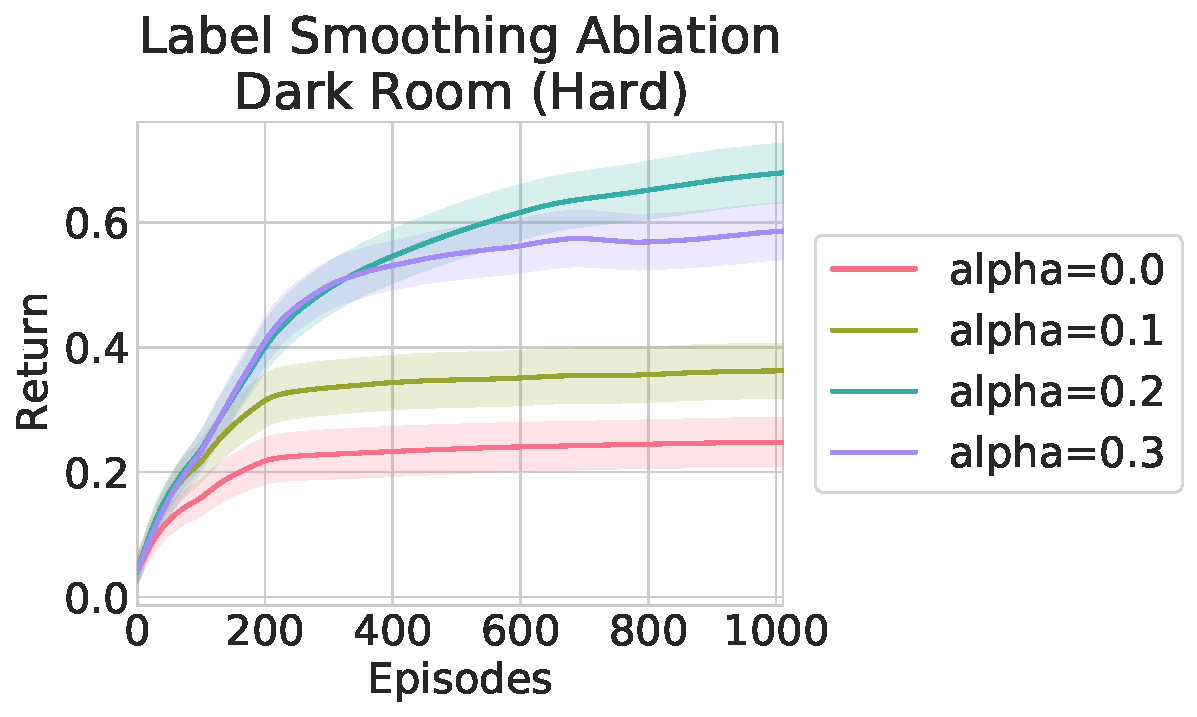
\includegraphics[width=0.55\textwidth]{assets/images/label_smoothing_ablation.pdf}
\caption{\name trained with different amounts of label smoothing on Dark Room (Hard).\small}
\label{fig:label_smoothing_ablation}
\end{figure}



\section{RL$^2$ network architecture: Transformer vs LSTM}

We compared using a transformer as the architecture for RL$^2$ instead of an LSTM. In Figure~\ref{fig:rl2_architecture_ablation}, we ran both transformer and LSTM RL$^2$ agents over the Dark Room environment. The curves shown are the best from a sweep over learning rate and unroll length hyperparameters. The transformer architecture is 4-layers with a model size of 256 and pre-norm layer normalization placement. While both agents reached a similar level of final performance, all RL$^2$ transformer models trained tended to be more unstable with the average return not as consistent as with an LSTM architecture. Given the poor performance of the transformer-based RL$^2$ on the simpler Dark Room setting, our other experimental settings used the LSTM.

\begin{figure}[h!]
\centering
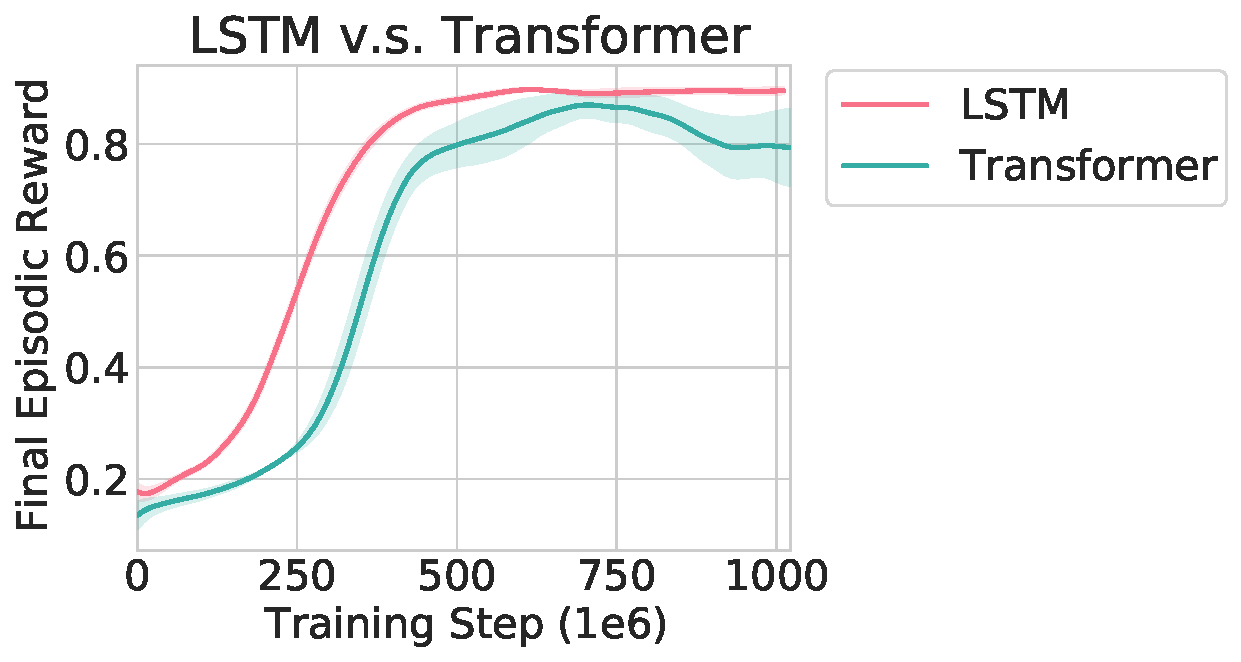
\includegraphics[width=0.6\textwidth]{assets/images/rl2_lstm_vs_transformer.pdf}
\caption{Comparison of LSTM and Transformer architecture for RL$^2$ agent on Dark Room. Each curve is averaged over 5 training seeds with the shaded area representing the standard error.}
\label{fig:rl2_architecture_ablation}
\end{figure}

\newpage

\section{Number of Training Tasks in Source Data}
\begin{figure}[h]
\centering
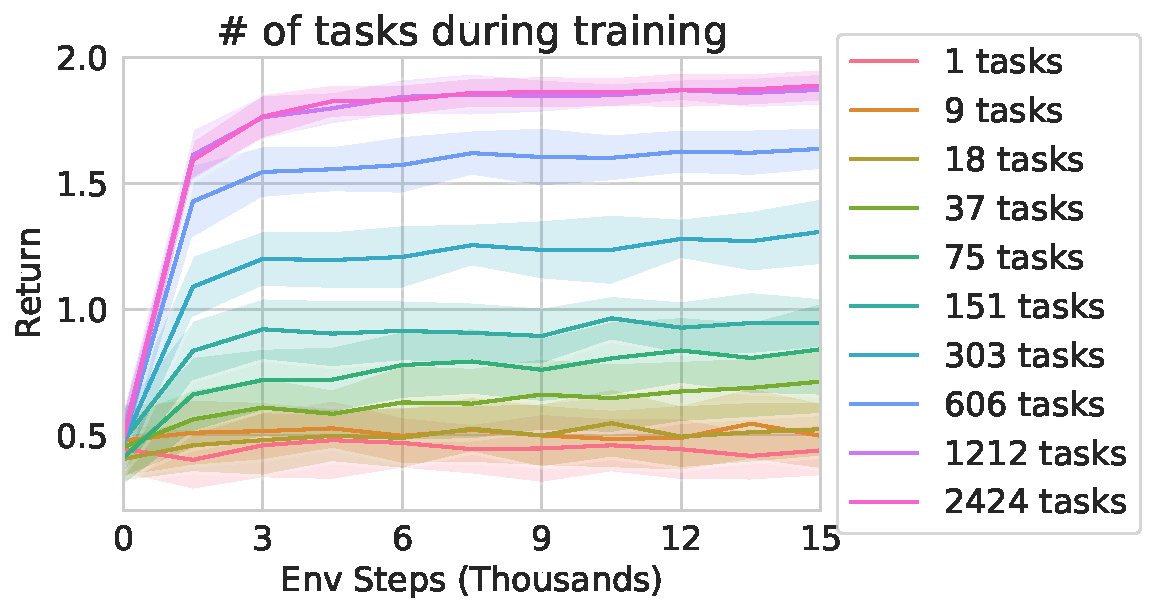
\includegraphics[width=0.6\textwidth]{assets/images/training_tasks_ablation_curves.pdf}
\caption{Algorithm distillation trained on different numbers of training tasks on Dark Key-to-Door evaluated on a fixed set of test tasks for 300 episodes of evaluation.}
\label{fig:ad_training_tasks}
\end{figure}



One interesting question is how many tasks \name needs to be trained on to learn an algorithm that generalizes to held out tasks. We trained \name on different numbers of Dark Key-to-Door training tasks and evaluated the resulting models on the same set of test tasks. Figure~\ref{fig:ad_training_tasks} shows the in-context learning plots for the resulting \name models on the set of test tasks. As a reminder, there are $81^2=6561$ unique Dark Key-to-Door tasks. Models trained on 1, 9 or 18 training tasks did not show any in-context learning on test tasks. While models trained on 37, 75 and 151 tasks did not achieve good performance overall, they did exhibit some in-context learning over the course of 300 episodes. The best models were trained on 1212 and 2424 tasks which corresponds to roughly $18\%$ and $37\%$ of the total number of tasks in the Dark Key-to-Door domain.

\section{Single-Stream \fullname}
\label{app:single_stream}


We provide more details around the experimental setup for the single-stream result shown in Fig.~\ref{fig:single_stream_ad}.
We showed in Fig.~\ref{fig:main_exps} that when \name is trained on data from a subset of the actors of a distributed source RL algorithm, the resulting model is more data efficient than the source algorithm. Here we confirm that \name can produce a faster algorithm than the one it was trained on in the single-stream setting. For this experiment we trained A3C on 2048 Dark Key-to-Door tasks for 2000 episodes each. We then trained \name on the resulting data while subsampling the learning histories by a factor of 10. More concretely, we took every 10th episode from each of the learning history, which resulted in a 200 episode compressed learning trajectory for each task. Figure~\ref{fig:single_stream_ad} compares the resulting \name model evaluated on a set of test tasks to the performance of the source algorithm on these tasks. The model learned by \name learns much faster than the source algorithm confirming that \fullname can turn a slow gradient-based algorithm into a much more data efficient in-context learning algorithm.

\section{Random mask}
\label{app:random_masking}
\begin{figure}[h]
\centering
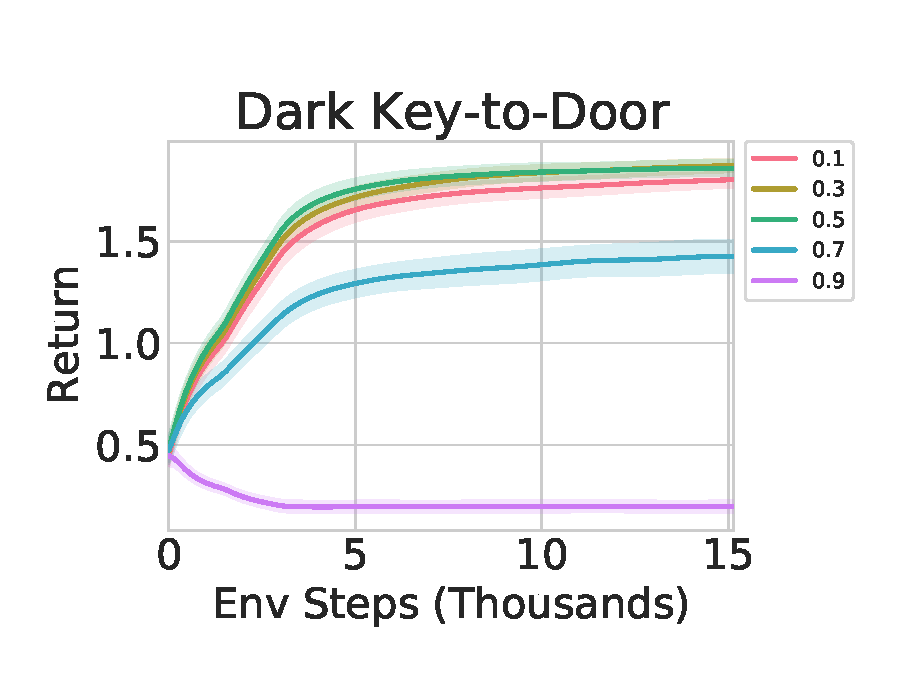
\includegraphics[width=0.5\textwidth]{assets/images/9x9_1g_mask.pdf}
\caption{Downstream performance of Algorithm Distillation with different values of random masking during training in 9x9 1 goal gridworld.}
\label{fig:9x9_1g_random_mask}
\end{figure}
During training, input tokens were randomly masked to avoid overfitting to training data. This plot shows the downstreams results on a 9x9 Dark Key-to-Door domain with different values of this random masking. Values of $0.3-0.5$ perform the best with the value of $0.3$ chosen for all experiments.

\section{AD network architecture: Transformer vs LSTM}
\label{app:transformer_vs_lstm}
Here we consider the importance of the Transformer architecture to the success of algorithm distillation (AD) by comparing to AD based off of an LSTM \citep{schm97lstm}. Specifically, the LSTM receives the concatenated embeddings of $\left(o_i, a_i, r_i\right)$ triplets up to the most recent time step $t-1$. The output of the LSTM is then concatenated with the current observation $o_t$ embedding and both are then fed through a multi-layer perceptron (MLP) policy torso to produce a distribution over the present action $a_t$. The LSTM hidden size (512), MLP depth (2), and MLP width (256) were swept and tuned by grid search based on downstream reward attainment.

Comparing Transformer AD and LSTM AD on the Dark Key-to-Door task, we find that both agents are capable of in-context learning, demonstrating that the success of AD is not tied to the underlying network architecture. However, we also find that the Transformer variant consistently outperforms the LSTM variant, which is why all other experiments in this paper employ the Transformer variant. This finding is consistent with the recent wider success of Transformer-based architectures over recurrent neural network (RNN)-based architectures in sequence prediction tasks.

\begin{figure}[h]
\centering
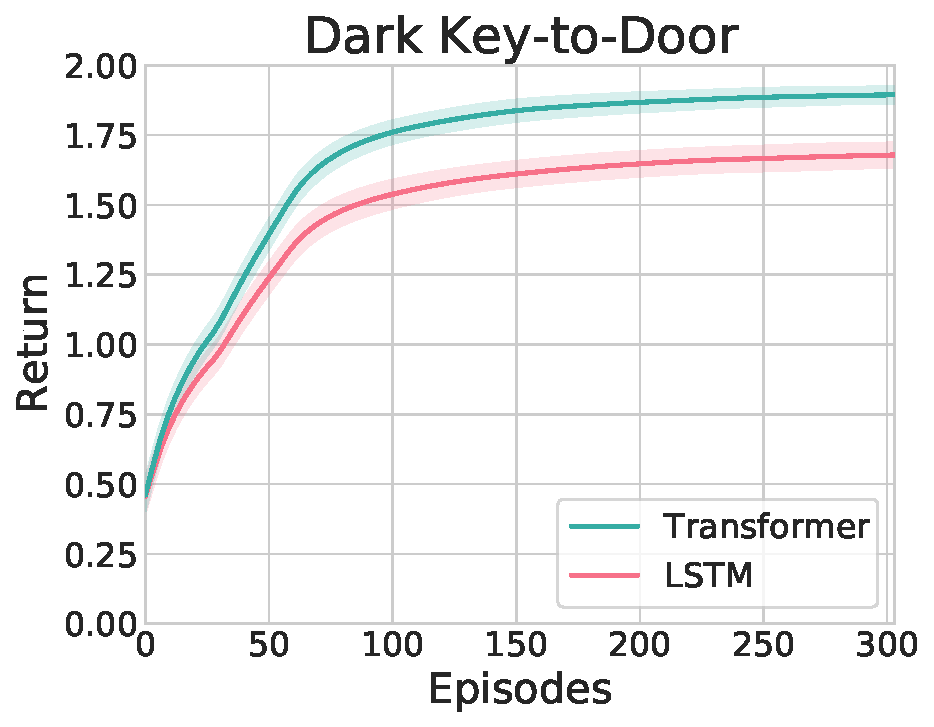
\includegraphics[width=0.45\textwidth]{assets/images/9x9_2g_transformer_vs_lstm.pdf}
\caption{Comparison between algorithm distillation with a Transformer and LSTM architecture on Dark Key-to-Door. Mean $\pm$ 1 standard deviation over 5 training seeds and 20 evaluation seeds. 300 episodes corresponds to 15k environment steps.}
\label{fig:9x9_2g_transformer_vs_lstm}
\end{figure}


\newpage


\section{\fullname Hyperparameters}
\label{app:ad_hypers}

%{\bf Architecture:} We use a 10-layer transformer architecture

\begin{table}[h!]
    \centering
    \scalebox{0.9}{
    \begin{tabular}{lcccc}
        \toprule
        Hyperparameter & Dark Room & Dark Room (Hard) & Dark Key-to-Door & Watermaze \\
        \midrule
        Embedding Dim. &  \multicolumn{4}{c}{64} \\
        Number of Layers & \multicolumn{4}{c}{4} \\
        Number of Heads & \multicolumn{4}{c}{4} \\
        Feedforward Dim. & \multicolumn{4}{c}{2048} \\
        Position Encodings & \multicolumn{4}{c}{Absolute} \\
        Layer Norm Placement & \multicolumn{4}{c}{Post Norm} \\
        Dropout Rate & \multicolumn{4}{c}{0.1} \\
        Attention Dropout Rate & 0.5 & 0 & 0.5 & 0.5 \\
        Sequence Mask Prob & 0.3 & 0.5 & 0.3 & 0.3 \\
        Label Smoothing $\alpha$  & 0 & 0.2 & 0 & 0 \\
        \bottomrule
    \end{tabular}}
    \caption{\fullname Architecture Hyperparameters.\small}
    \label{tab:arch_hypers}
    \small
\end{table}

\begin{table}[h]
    \centering
    \scalebox{0.9}{
    \begin{tabular}{lcc}
        \toprule
         Hyperparameter & Value \\ \midrule
         Batch Size & 128 \\
         Optimizer & Adam \\
         $\beta_1$ & 0.9 \\
         $\beta_2$ & 0.99 \\
         Gradient Clip Norm Threshold & 1 \\ \midrule
         Learning Rate Schedule & Cosine Decay \\
         Initial Value & 2e-6 \\
         Peak Value & 3e-4 \\
         \bottomrule
    \end{tabular}}
    \caption{\fullname Optimization Hyperparameters.\small}
    \label{tab:opt_hypers}
    \small
\end{table}

\begin{table}[h]
    \centering
    \scalebox{0.9}{
    \begin{tabular}{lcc}
        \toprule
         Layer & Hyperparameter & Value \\ \midrule
         \it{Conv Block} & \\
         \multirow{3}{4em}{Conv} &  Channel & 128 \\
          &  Kernel & 5 \\
          &  Stride & 2 \\
         \multirow{2}{5em}{BatchNorm} & Decay Rate & 0.999 \\
         & eps & 1e-5 \\
         Activation & - & ReLU \\
         \multirow{2}{7em}{Max Pooling} & Kernel & 2 \\
         & Stride & 2 \\
         Dropout & Rate & 0.2 \\ \midrule
         \it{Network} & \\
         Conv Blocks & - & 3 \\
         Final Linear Layer & Units & 256 \\
         \bottomrule
    \end{tabular}}
    \caption{Watermaze Image Encoder Hyperparameters.\small}
    \label{tab:watermaze_enc_hypers}
    \small
\end{table}

\newpage
\section{Source RL Algorithm Hyperparameters}
\label{app:rl_hypers}

\subsection{Dark Environments}


\begin{table}[h]
    \centering
    \scalebox{0.9}{
    \begin{tabular}{lcc}
        \toprule
         Hyperparameter & Value \\ \midrule
         Batch Size (Num. Actors) & 100 \\
         $\lambda$ & 0.95 \\
         Agent Discount & 0.99 \\
         Entropy Bonus Weight & 0.01 \\
         MLP Layers & 3 \\
         MLP Hidden Dim & 128 \\
         Optimizer & Adam \\
         $\beta_1$ & 0.9 \\
         $\beta_2$ & 0.999 \\
         $\epsilon$ & 1e-6 \\
         Learning Rate & 1e-4 \\
         \bottomrule
    \end{tabular}}
    \caption{Source A3C Algorithm Hyperparameters for Dark Environments.\small}
    \label{tab:watermaze_source_algo}
    \small
\end{table}

\subsection{ DMLab Watermaze}

\begin{table}[h]
    \centering
    \scalebox{0.9}{
    \begin{tabular}{lcc}
        \toprule
         Hyperparameter & Value \\ \midrule
         Batch Size & 8 \\
         Rollout Length & 40 \\
         Rollout Overlap & 31 \\
         Number of Actors & 16 \\
         Reply Buffer Capacity & 1e5 \\
         Offline Data Fraction & 0.7 \\
         $\lambda$ & 0.75 \\
         $\epsilon$ & 0.01 \\
         Agent Discount & 0.9 \\
         Target Update Period & 50 \\ \midrule
         ResNet Channels & [32, 64, 64] \\
         ResNet Kernels & [3, 3, 3] \\
         ResNet Strides & [1, 1, 1] \\
         Pool Kernels & [3, 3, 3] \\
         Pool Strides & [2, 2, 2] \\ \midrule
         Optimizer & Adam \\
         $\beta_1$ & 0.9 \\
         $\beta_2$ & 0.999 \\
         $\epsilon$ & 1e-6 \\
         Gradient Clip Norm Threshold & 10 \\
         Learning Rate & 1e-4 \\
         \bottomrule
    \end{tabular}}
    \caption{Source DQN(Q-$\lambda$) Algorithm Hyperparameters for Watermaze.\small}
    \label{tab:watermaze_source_algo}
    \small
\end{table}

\newpage

\section{RL$^2$ Hyperparameters}
\label{app:rl2_hypers}

\begin{table}[h]
    \centering
    \begin{tabular}{lc}
    \toprule
    Hyperparameter & Value \\ \midrule
    RL Algorithm & A3C \\
    Learning Rate & 3e-4 \\
    Batch Size & 256 \\
    Unroll Length & 20 \\
    LSTM Hidden Dim. & 256 \\
    LSTM Number of Layers & 2 \\
    Episodes Per Trial & 10 \\
    \bottomrule
    \end{tabular}
    \caption{RL$^2$ Hyperparameters used in ``Dark'' Environments.\small}
    \small
\end{table}

\begin{table}[h]
    \centering
    \begin{tabular}{lc}
    \toprule
    Hyperparameter & Value \\ \midrule
    RL Algorithm & DQN(Q-$\lambda$) \\
    Learning Rate & 1e-4 \\
    Batch Size & 96 \\
    Unroll Length & 40 \\
    LSTM Hidden Dim. & 256 \\
    LSTM Number of Layers & 1 \\
    Episodes Per Trial & 30 \\
    \bottomrule
    \end{tabular}
    \caption{RL$^2$ Hyperparameters used in the Watermaze Environment.\small}
    \small
\end{table}


\newpage 
\section{Attention Maps}


\begin{figure}[h]
\centering
% \begin{subfigure}{.5\textwidth}
  \centering
  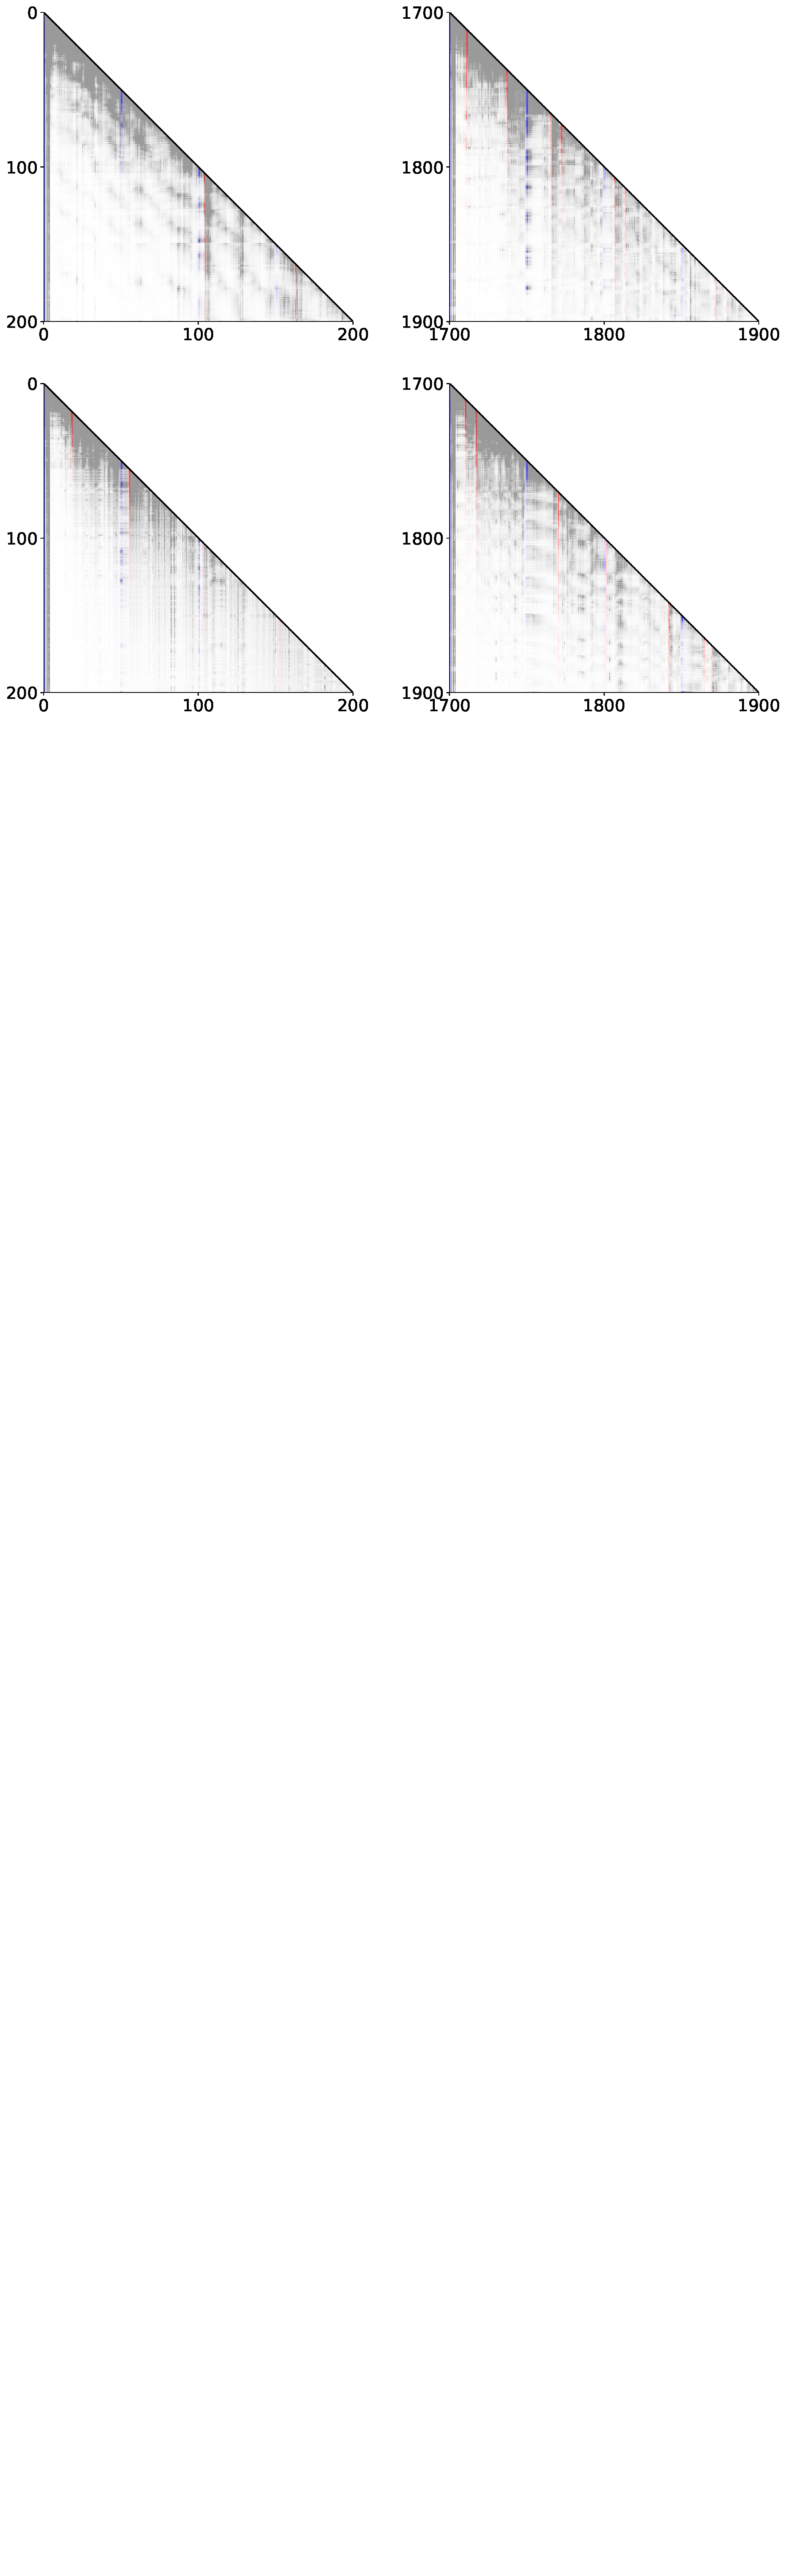
\includegraphics[width=1.0\textwidth]{assets/images/attention_4.pdf}
  \caption{Attention maps for \name from five separate seeds. White and gray colors correspond to low and high attention. Red and blue colors indicate that those transitions correspond to an episode restart and a positive reward token, respectively. The left column plots attention for an AD transformer after 200 time-steps of evaluation (when the context is initially filled). The right column plots attention after 1900 steps (38 episodes) of evaluation. Each episode has a length of 50 steps. From these patterns, it is evident that \name attends to tokens across several episodes to predict its next action.}
  \label{fig:sub1}

\label{fig:test}
\end{figure}